%
% NOTE -- ONLY EDIT THE .Rnw FILE!!!  The .tex file is
% likely to be overwritten.
%
%\VignetteIndexEntry{Using Chromosome Bands as Categories}
%\VignetteDepends{ALL, hgu95av2.db, annotate, genefilter, SNPchip,
% geneplotter, limma, lattice, graph}
%\VignetteKeywords{graphs, visualization}
%\VignettePackage{Category}
\documentclass[11pt]{article}

\usepackage{times}
\usepackage{hyperref}

\usepackage[authoryear,round]{natbib}
\usepackage{times}
\usepackage{comment}

\textwidth=6.2in
\textheight=8.5in
%\parskip=.3cm
\oddsidemargin=.1in
\evensidemargin=.1in
\headheight=-.3in

\newcommand{\Rclass}[1]{\textit{``#1''}}
\newcommand{\Rpackage}[1]{{\textsf{#1}}}
\newcommand{\Rfunction}[1]{{\texttt{#1()}}}


\usepackage{Sweave}


\bibliographystyle{plainnat}

\title{Using Categories defined by Chromosome Bands}
\author{D. Sarkar, S. Falcon, R. Gentleman}
\date{August 7, 2008}

\begin{document}
\Sconcordance{concordance:ChromBand.tex:ChromBand.Rnw:%
1 99 1 1 2 1 0 4 1 1 2 1 0 4 1 3 0 1 2 7 1 1 19 24 1 1 2 1 0 1 2 2 1 1 %
2 1 1 3 0 1 2 3 1 1 2 1 0 1 2 1 0 1 2 1 0 1 2 4 0 1 2 10 1 1 5 4 0 1 1 %
3 0 1 2 3 1 1 3 2 0 1 2 1 0 1 1 3 0 1 2 3 1 1 2 1 0 2 1 1 2 4 0 1 2 8 1 %
1 2 1 0 7 1 1 2 1 1 4 0 1 3 2 1 1 2 1 0 3 1 4 0 1 3 158 1 1 17 18 0 1 2 %
2 1 1 14 17 0 1 4 2 1 1 37 35 0 1 2 1 1 1 7 9 0 1 3 11 1 1 8 7 0 1 2 1 %
1 3 0 1 2 2 1 1 2 1 0 1 1 3 0 1 2 2 1 1 2 1 0 1 1 30 0 1 2 1 1 26 0 1 2 %
47 1 1 16 18 0 1 5 63 1 1 9 8 0 4 1 3 0 1 2 1 3 1 0 1 1 1 2 56 0 1 1 37 %
0 1 4 9 1 1 2 1 0 1 2 4 0 1 5 22 1}


\maketitle

% \section{Introduction}

% Categories or gene sets (mappings of genes to classes) are becoming an
% important tool for the analysis of microarray data.  The
% \Rpackage{Category} package enables category based analysis
% approaches; this vignette demonstrates tools that allow the use of
% categories derived from chromosome bands.  Although in normal
% multi-cellular eukaryotic organisms there is generally not a strong
% relationship between chromosomal location and expression (notable
% exceptions being the HOX family of genes), there are a number of
% diseases where either genetic (amplification or deletion of DNA) or
% epigenetic (methylation or demethylation) events will result in
% changes in gene expression that can be associated with particular
% chromosomal locations.  Our goal is to identify genomic regions with
% systematic alterations in gene expression levels.  

% We consider the use
% of chromosome bands as gene sets to address this question.


% how microarray gene expression
% data can be analyzed using  as gene sets, and how the
% hierarchical nature of that information can be used in systematic
% statistical testing.

% This vignette describes tools in the
% \Rpackage{Category} package that work with gene sets derived from
% chromosomal location.



\section{Chromosome bands}

Typically, in higher organisms, each chromosome has a centromere and
two arms.  The short arm is called the p arm and the longer arm the q
arm.  Chromosome bands (see Figure~\ref{fig:chr12ideogram}) are
identified by differential staining, usually with Giemsa-based stains,
and many disease-related defects have been mapped to these bands; such
mappings have played an important role in classical cytogenetics.
With the availability of complete sequences for several genomes, there
have been efforts to link these bands with specific sequence locations
\citep{FureyHaussler}.  The estimated location of the bands in the
reference genomes can be obtained from the UCSC genome browser, and
data linking genes to particular bands can be obtained from a variety
of sources such as the NCBI.  This vignette demonstrates tools that
allow the use of categories derived from chromosome bands, that is,
the relevant categories are determined \textit{a priori} by a mapping
of genes to chromosome bands.

Figure~\ref{fig:chr12ideogram} shows an ideogram of human chromosome
12, with the band 12q21 shaded.  As shown in the figure, 12q21 can be
divided into more granular levels 12q21.1, 12q21.2, and 12q21.3.
12q21.3 can itself be divided at an even finer level of resolution
into 12q21.31, 12q21.32, and 12q21.33.  Moving towards less granular
bands, 12q21 is a part of 12q2 which is again a part of 12q.  We take
advantage of this nested structure of the bands in our analysis.
\begin{Schunk}
\begin{Sinput}
> library("Category")
> library("ALL")
> library("hgu95av2.db")
> library("annotate")
> library("genefilter")
> ##library("SNPchip")
> library("karyoploteR")
> library("geneplotter")
> library("limma")
> library("lattice")
> library("graph")
\end{Sinput}
\end{Schunk}




%
\begin{figure}[tb]
\begin{center}
%
\end{center}
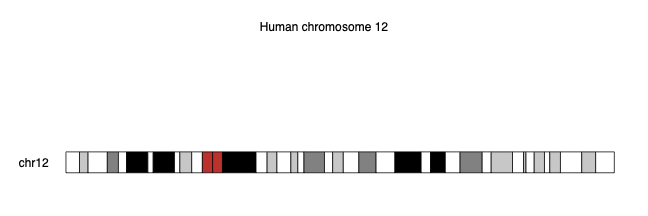
\includegraphics[width=.98\textwidth]{chr12ideogram}
\caption{Ideogram for human chromosome 12.  The p arm is on the left,
  the q arm is on the right, and the centromere is indicated by a
  notch.  The shaded bands together represent 12q21.  This band is
  composed of three sub-bands: 12q21.1, 12q21.2, and 12q21.3.  The
  last of these is composed of sub-sub-bands 12q21.31, 12q21.32, and
  12q21.33. }
\label{fig:chr12ideogram}
\end{figure}
%


\section{Data Preparation}

For illustration, we use a microarray dataset \citep{Chiaretti2005}
from a clinical trial in acute lymphoblastic leukemia (ALL).  The data
are described in Chapter~2 of \cite{biocCaseStudies}.  For the
analysis presented here, we consider the comparison of two subsets:
patients identified as having a BCR/ABL gene fusion present, typically
as a result of a translocation of chromosomes 9 and 22 (labeled
BCR/ABL), and those that have no observed cytogenetic abnormalities
(labeled NEG).  The full dataset is available in the \Rpackage{ALL}
package, and the relevant subset of the data can be obtained by
%
\begin{Schunk}
\begin{Sinput}
> data(ALL, package="ALL")
> subsetType <- "BCR/ABL"
> Bcell <- grep("^B", as.character(ALL$BT))
> bcrAblOrNegIdx <- which(as.character(ALL$mol.biol) %in% c("NEG", subsetType))
> bcrAblOrNeg <- ALL[, intersect(Bcell, bcrAblOrNegIdx)]
> bcrAblOrNeg$mol.biol <- factor(bcrAblOrNeg$mol.biol)
\end{Sinput}
\end{Schunk}
%
We also create relevant annotation maps to go from feature names to
Entrez ID, gene symbol, and chromosome band.
%
\begin{Schunk}
\begin{Sinput}
> annType <- c("db", "env")
> entrezMap <- getAnnMap("ENTREZID", annotation(bcrAblOrNeg),
+                        type=annType, load=TRUE)
> symbolMap <- getAnnMap("SYMBOL", annotation(bcrAblOrNeg),
+                        type=annType, load=TRUE)
> bandMap <- getAnnMap("MAP", annotation(bcrAblOrNeg),
+                      type=annType, load=TRUE)
\end{Sinput}
\end{Schunk}
%


We applied a non-specific filter to the dataset to remove probesets
lacking the desired annotation as well as those with an interquartile
range (IQR) below the median IQR, as probesets with little variation
across samples are uninformative.  We also ensured that each Entrez
Gene identifier maps to exactly one probeset by selecting the probeset
with the largest IQR when two or more probesets map to the same Entrez
Gene ID.
%
\begin{Schunk}
\begin{Sinput}
> filterAns <- nsFilter(bcrAblOrNeg,
+                       require.entrez = TRUE, 
+                       remove.dupEntrez = TRUE, 
+                       var.func = IQR, var.cutoff = 0.5)
> nsFiltered <- filterAns$eset
\end{Sinput}
\end{Schunk}
%
We also remove probesets with no gene symbol, as well as those with no
mapping to a chromosome band.
%
\begin{Schunk}
\begin{Sinput}
> hasSYM <- sapply(mget(featureNames(nsFiltered), symbolMap, ifnotfound=NA),
+                  function(x) length(x) > 0 && !is.na(x[1]))
> hasMAP <- sapply(mget(featureNames(nsFiltered), bandMap, ifnotfound=NA),
+                  function(x) length(x) > 0 && !is.na(x[1]))
> nsFiltered <- nsFiltered[hasSYM & hasMAP, ]
\end{Sinput}
\end{Schunk}
%
We define the \textit{gene universe} to be the subset of genes that
remain after this filtering.
%
\begin{Schunk}
\begin{Sinput}
> affyUniverse <- featureNames(nsFiltered)
> entrezUniverse <- unlist(mget(affyUniverse, entrezMap))
> names(affyUniverse) <- entrezUniverse
> if (any(duplicated(entrezUniverse)))
+     stop("error in gene universe: can't have duplicate Entrez Gene Ids")
\end{Sinput}
\end{Schunk}




We assessed differential expression between the BCR/ABL and
NEG groups using an empirical Bayes approach, as implemented in the
software package \Rpackage{limma}~\citep{limma}, yielding an
attenuated $t$-statistic for each gene.
%
\begin{Schunk}
\begin{Sinput}
> design <- model.matrix(~ 0 + nsFiltered$mol.biol)
> colnames(design) <- c("BCR/ABL", "NEG")
> contr <- c(1, -1) ## NOTE: we thus have BCR/ABL w.r.t NEG
> fm1 <- lmFit(nsFiltered, design)
> fm2 <- contrasts.fit(fm1, contr)
> fm3 <- eBayes(fm2)
> ttestLimma <- topTable(fm3, number = nrow(fm3), adjust.method = "none")
> ttestLimma <- ttestLimma[featureNames(nsFiltered), ]
> tstats <- ttestLimma$t
> names(tstats) <- entrezUniverse[rownames(ttestLimma)]
> ##
\end{Sinput}
\end{Schunk}
%
We used a $p$-value cutoff of $0.01$ to identify a list of potentially
differentially expressed genes.
\begin{Schunk}
\begin{Sinput}
> ttestCutoff <- 0.01
> smPV  <- ttestLimma$P.Value < ttestCutoff
> pvalFiltered <- nsFiltered[smPV, ]
> selectedEntrezIds <- unlist(mget(featureNames(pvalFiltered), entrezMap))
> ##
\end{Sinput}
\end{Schunk}




% \section{Types of tests}

% % We describe the use of marginal and conditional Hypergeometric tests
% % to identify unusual chromosome bands, and a contingency table approach
% % to perform local tests.  We also describe an implementation of GSEA
% % that we use to perform marginal and conditional tests.

% We explore three approaches for using the chromosome band gene sets in
% our example analysis: Hypergeometric testing, a generic contingency
% table approach that allows for testing multiple gene sets
% simultaneously, and gene set enrichment analysis (GSEA).  

% Hypergeometric and contingency table testing rely on a list of
% selected genes, created by artificially dividing genes into two
% classes (differentially expressed or not).  The GSEA approach does not
% rely on the identification of differentially expressed genes, but
% rather on computed per-gene summary statistics.  

% To motivate these analytical approaches, we observe that there are two
% important features of gene sets based on chromosome bands:
% (1) the bands are nested hierarchically, and (2) they almost form a
% partition (for most species almost all genes appear in only one
% location in the genome).

% The first observation is important because it allows us to perform
% conditional tests.  When testing a particular sub-band, we are
% interested in knowing whether genes annotated at that sub-band are
% unusual relative to some larger set of genes.  If we have already
% answered that question in the affirmative for one or more
% sub-sub-bands, then to declare the band under consideration unusual,
% we may desire evidence for that assertion beyond that furnished by the
% unusual sub-sub-bands---such tests are conditional tests.
% \citet{Falcon-GOstats} address this question in the context of
% Hypergeometric tests for over-representation of GO terms ~\citep{GO}.


% The second observation suggests that it is possible to improve upon
% methods that test each band separately.  One can either treat each
% chromosome as a unit, or, since it is unlikely that any important
% event (amplification, deletion, methylation) spans the centromere in
% humans, divide the data into 48 groups (one for each half of each
% chromosome).  Then, within each group of gene sets, one can determine
% the number of top-level chromosome bands, $K_c$, for each chromosome
% arm $c$ and perform a standard 2 by $K_c$ contingency table
% analysis. This approach reduces the issues that arise due to multiple
% testing.  If one of these tests is rejected, other contingency tables
% constructed from the sub-band annotations can help identify the
% location(s) most responsible for the rejection.





\section{Methods}



There are two important features of gene sets based on chromosome
bands: (1) the bands are nested hierarchically, and (2) they almost
form a partition (for most species almost all genes appear in only one
location in the genome).  This naturally leads to two different
dichotomies in approaches to testing: one is a top-down versus a
bottom-up approach, and the other contrasts local tests with global
tests.  We use human chromosome 12 as an example to describe these
approaches.  Users will need to identify which of the approaches best
align with their objectives and then make use of the software
appropriately.

Conceptually one can start a sequential testing approach either at the
most coarse level of organization (probably the level of the arm: p or
q), or the most specific level (that of sub-sub-bands). In the
top-down approach, one first tests the hypothesis of interest on a
coarse level of organization, and if rejected, the next level of
organization is considered.  For example, we might first consider the
band 12q21, and if that hypothesis is rejected, test each of the
sub-bands 12q21.1, 12q21.2, and 12q21.3. If the hypothesis for 12q21.3
is rejected, then we may subsequently examine each of 12q21.31,
12q21.32, and 12q21.33.

The bottom-up approach differs in that we begin at the most granular
level and move upward, amalgamating adjacent bands at each level.  The
bottom-up approach is easier to put into a conditional hypothesis
testing framework.  Our initial null hypotheses involve the smallest,
or most granular bands, and if there is evidence that these are
unusual (i.e., we reject the null hypothesis) then moving to a larger,
or less granular, band requires additional information to declare it
significant, over and above what we have used to identify the smaller
band.  In our example, we would first test 12q21.31, 12q21.32, and
12q21.33, and then move up and test 12q21.3.  If one or more of the
three sub-bands had been declared significant, we would exclude the
evidence from genes annotated in those sub-bands when testing the
coarser band.

It is important to note that the top-down versus bottom-up approaches
represent a fundamental trade-off between false positive and false
negative errors.  The bottom-up approach necessarily involves
performing a larger number of tests, yielding a correspondingly larger
absolute number of false positives for a given false positive rate at
which each individual test is controlled.  The top-down approach cuts
down on the number of false positives by starting with fewer top-level
tests, and performing further tests at sublevels only when a top-level
test is rejected.  The disadvantage to this approach is loss of power
to detect real departures that are localized to a sub-level, a
phenomenon commonly illustrated using Simpson's paradox
\citep[see, e.g.,][]{Simpson1982}.

Whether a test is local or global is a different question, orthogonal
to that of top-down or bottom-up.  There are two distinct but
potentially relevant questions that may be of interest.  The first is
whether genes in a particular gene set are ``different'' relative to
all other genes under consideration.  For a Hypergeometric test, this
question may be formalized as whether the proportion of interesting
genes in 12q21 is different from the proportion of interesting genes
in the rest of the genome, or equivalently, whether membership in
12q21 is independent of being selected.  Such tests are
\textit{global} in the sense that all genes in the gene universe are
used to determine whether or not genes at a location are unusual or
not.  An alternative is to ask whether genes in a genomic location are
different relative to other genes in some meaningfully defined
neighbourhood.  Such a test can be performed simply by restricting the
gene universe to a suitable subset; for example, when testing 12q21,
we may only consider genes in 12q.  A more natural approach is to use
a $2 \times 3$ contingency table to test the hypothesis that the
proportion of interesting genes is the same in 12q21, 12q22, and
12q23.  Both these tests are \textit{local} in the sense that only
nearby genes are used.  

Contingency table tests are inherently local and although they do not
naturally extend to conditional testing, we can use a top-down
approach to test at various resolutions.  Such tests can be performed
by the \Rfunction{cb\_contingency} function, which we do not discuss in
this vignette.  Instead, we focus on the bottom-up approach, which
allows for conditional testing.


% \section{Analysis}

% We begin by building a graph representing the tree structure of the
% chromosome band annotations for the genes in the gene universe, as
% such a representation is natural and convenient.  The chromosome band
% annotation for each gene in the universe is added to the tree along
% with all parent bands up to the chromosome level.  For example, if one
% of the genes is annotated at 12q21.1, we add the following nodes to
% the tree if they are not already present: 12q21, 12q2, 12q, and 12.
% As a consequence of the nesting structure of the bands, each parent
% band inherits the gene annotations of its children.  This situation is
% similar to a graph of GO terms where the \textit{is-a} relationship
% implies inheritance of gene annotations by less specific terms from
% more specific ones.

\section{Utility functions}

We first define a few utility functions that we subsequently use in
presentation.  The \Rfunction{chrSortOrder} function reorders rows of
data frame for display in a natural order.
\begin{Schunk}
\begin{Sinput}
> chrSortOrder <- function(df) {
+     chrs <- sub("([^pq]+).*$", "\\1", rownames(df))
+     xyIdx <- chrs %in% c("X", "Y")
+     xydf <- NULL
+     if (any(xyIdx)) {
+         chrs <- chrs[!xyIdx]
+         xydf <- df[xyIdx, ]
+         df <- df[!xyIdx, ]
+     }
+     ord <- order(as.integer(chrs), rownames(df))
+     df <- df[ord, ]
+     if (!is.null(xydf))
+       df <- rbind(df, xydf)
+     df
+ }
\end{Sinput}
\end{Schunk}
%
The \Rfunction{gseaTstatStripplot} function creates a comparative
strip plot of the $t$-statistics for specified bands.
\begin{Schunk}
\begin{Sinput}
> gseaTstatStripplot <- function(bands, g, ..., include.all = FALSE)
+ {
+     chroms <- c(1:22, "X", "Y")
+     chromArms <- c(paste(chroms, "p", sep=""), paste(chroms, "q", sep=""))
+     egid <- lapply(nodeData(g, bands), "[[", "geneIds")
+     if (include.all) {
+         egid$All <- 
+             unique(unlist(lapply(nodeData(g)[chromArms], "[[", "geneIds")))
+     }
+     tdf <- do.call(make.groups, lapply(egid, function(x) tstats[x]))
+     stripplot(which ~ data, tdf, jitter = TRUE, ...)
+ }
> 
> 
\end{Sinput}
\end{Schunk}

The \Rfunction{esetBWPlot} function creates box-and-whisker plots for
every gene in an \Rclass{ExpressionSet}.
\begin{Schunk}
\begin{Sinput}
> esetBWPlot <- function(tmpSet, ..., layout=c(1, nrow(emat)))
+ {
+     emat <- exprs(tmpSet)
+     pd <- pData(tmpSet)
+     probes <- rownames(emat)
+     syms <- 
+         sapply(mget(probes, hgu95av2SYMBOL, ifnotfound=NA),
+                function(x) if (all(is.na(x))) "NA" else as.character(x)[1])
+     selectedAffy <- 
+         probes %in% affyUniverse[selectedEntrezIds]
+     symsSelected <- syms[selectedAffy]
+     symsWithStatus <- 
+         paste(syms, 
+               ifelse(selectedAffy, "*", ""), 
+               sep = "")
+     pdat <- 
+         cbind(exprs=as.vector(emat),
+               genes=factor(probes, levels = probes, labels = syms),
+               pd[rep(seq_len(nrow(pd)), each=nrow(emat)), ])
+     pdat <- transform(pdat, genes = reorder(genes, exprs))
+     panels.to.shade <- levels(pdat$genes) %in% symsSelected
+     bwplot(mol.biol ~ exprs | genes, data=pdat, 
+            layout = layout,
+            auto.key=TRUE,
+            scales=list(x=list(log=2L)),
+            xlab="Log2 Expression",
+            panels.to.shade = panels.to.shade,
+            panel = function(..., panels.to.shade) {
+                if (panels.to.shade[packet.number()]) 
+                    panel.fill(col = "lightgrey")
+                panel.bwplot(...)
+            },
+            strip=FALSE,
+            strip.left=TRUE, ...)
+ }
> g1 <- makeChrBandGraph(annotation(nsFiltered), univ=entrezUniverse)
> ct <- ChrBandTreeFromGraph(g1)
> subsetByBand <- function(eset, ct, band) {
+     egIDs <- unlist(nodeData(ct@toChildGraph, n=band, 
+                              attr="geneIds"), use.names=FALSE)
+     wantedProbes <- affyUniverse[as.character(egIDs)]
+     eset[intersect(wantedProbes, featureNames(eset)), ]
+ }
> 
\end{Sinput}
\end{Schunk}

\section{Hypergeometric Testing}

We use a method similar to that described in~\citet{Falcon-GOstats} to
conditionally test for over-representation of chromosome bands in the
selected gene list.  A test is set up by creating a suitable object of
class \Rclass{ChrMapHyperGParams}.  We first create an object to
perform a standard Hypergeometric analysis, treating each chromosome
band independently, and then modify a copy to represent a conditional
Hypergeometric computation.
%
%
\begin{Schunk}
\begin{Sinput}
> params <- new("ChrMapHyperGParams",
+               conditional=FALSE,
+               testDirection="over",
+               universeGeneIds=entrezUniverse,
+               geneIds=selectedEntrezIds,
+               annotation="hgu95av2",
+               pvalueCutoff=0.05)
> paramsCond <- params
> paramsCond@conditional <- TRUE
\end{Sinput}
\end{Schunk}
%
The test computations are performed by
%
\begin{Schunk}
\begin{Sinput}
> hgans <- hyperGTest(params)
> hgansCond <- hyperGTest(paramsCond)
\end{Sinput}
\end{Schunk}
%
The results can be summarized by
% 
\begin{Schunk}
\begin{Sinput}
> sumUn <- summary(hgans, categorySize=1)
> chrSortOrder(sumUn)
\end{Sinput}
\begin{Soutput}
   ChrMapID       Pvalue OddsRatio   ExpCount Count Size
1   14q22.2 0.0005784156 22.692958  0.4907724     4    6
2    7q31.2 0.0047908084 16.971910  0.4089770     3    5
3    9q21.1 0.0062117150  7.556808  0.8179540     4   10
4     13q31 0.0066733711       Inf  0.1635908     2    2
5   13q31.1 0.0066733711       Inf  0.1635908     2    2
6      6p23 0.0066733711       Inf  0.1635908     2    2
7    9q33.2 0.0090032012 11.311798  0.4907724     3    6
8    2p22.2 0.0148085762  8.481742  0.5725678     3    7
9  12q21.33 0.0189339982 22.571429  0.2453862     2    3
10   2q31.3 0.0189339982 22.571429  0.2453862     2    3
11   4q22.1 0.0189339982 22.571429  0.2453862     2    3
12    14q22 0.0197575131  3.780603  1.6359080     5   20
13    12q14 0.0222758094  6.783708  0.6543632     3    8
14      6q2 0.0229391129  2.164685  5.6438824    11   69
15  12q21.3 0.0358280017 11.282913  0.3271816     2    4
16     4q22 0.0358280017 11.282913  0.3271816     2    4
17 10p11.22 0.0358280017 11.282913  0.3271816     2    4
18 12q13.11 0.0358280017 11.282913  0.3271816     2    4
19   6q24.2 0.0358280017 11.282913  0.3271816     2    4
20        9 0.0419943288  1.624759 12.5146958    19  153
21     1p21 0.0422279373  4.843098  0.8179540     3   10
22    20p12 0.0422279373  4.843098  0.8179540     3   10
23 22q11.23 0.0422279373  4.843098  0.8179540     3   10
24       6q 0.0439995864  1.808967  7.7705628    13   95
25  1p36.11 0.0446151403  3.481690  1.3905218     4   17
\end{Soutput}
\begin{Sinput}
> sumCond <- summary(hgansCond, categorySize=1)
> chrSortOrder(sumCond)
\end{Sinput}
\begin{Soutput}
   ChrMapID       Pvalue OddsRatio   ExpCount Count Size
1   14q22.2 0.0005784156 22.692958  0.4907724     4    6
2    7q31.2 0.0047908084 16.971910  0.4089770     3    5
3    9q21.1 0.0062117150  7.556808  0.8179540     4   10
4   13q31.1 0.0066733711       Inf  0.1635908     2    2
5      6p23 0.0066733711       Inf  0.1635908     2    2
6    9q33.2 0.0090032012 11.311798  0.4907724     3    6
7    2p22.2 0.0148085762  8.481742  0.5725678     3    7
8  12q21.33 0.0189339982 22.571429  0.2453862     2    3
9    2q31.3 0.0189339982 22.571429  0.2453862     2    3
10   4q22.1 0.0189339982 22.571429  0.2453862     2    3
11    12q14 0.0222758094  6.783708  0.6543632     3    8
12      6q2 0.0229391129  2.164685  5.6438824    11   69
13 10p11.22 0.0358280017 11.282913  0.3271816     2    4
14 12q13.11 0.0358280017 11.282913  0.3271816     2    4
15   6q24.2 0.0358280017 11.282913  0.3271816     2    4
16        9 0.0419943288  1.624759 12.5146958    19  153
17     1p21 0.0422279373  4.843098  0.8179540     3   10
18    20p12 0.0422279373  4.843098  0.8179540     3   10
19 22q11.23 0.0422279373  4.843098  0.8179540     3   10
20  1p36.11 0.0446151403  3.481690  1.3905218     4   17
\end{Soutput}
\end{Schunk}
%


For the standard test, the structure of the chromosome band graph is
ignored and a Hypergeometric test is applied to each band
independently.  For the conditional test, the hierarchical
relationship among the bands as represented by the graph is used in
the computation.  The highest-resolution bands (those with no children
in the graph) are tested first.  Testing proceeds with the bands whose
children (sub-bands) have already been tested.  For these bands, the
gene annotations that are inherited from significant child nodes
(children with $p$-value smaller than the specified cutoff) are
removed prior to testing to yield a conditional test.

The effect of the conditional test is illustrated by examining the
results for 14q and its sub-bands.  In the standard test, we see that
14q22 and 14q22.2 both have a significant $p$-value.  In the
conditional test, only 14q22.2 remains.  The conclusion is that there
is not enough additional evidence beyond that provided by 14q22.2 to
mark 14q22 as significant.







\section{GSEA using linear models}



GSEA is a popular method that can be used to assess whether or not
particular gene sets are associated with a phenotype of interest
\citep{Subramanian2005, Tian2005, JiangGent2007}.  Most applications
of this method do not explicitly deal with structure of the gene sets,
but when analyzing chromosomal location such methods are desirable.
We present a simple approach that is similar in spirit to traditional
GSEA, and generalizes nicely to accommodate nested categories.
Consider the situation where gene $i$ has an associated measure of
differential expression $y_i$; for example, an attenuated
$t$-statistic derived from a differential expression analysis such as
\Rpackage{limma}~\citep{limma}.  Given a particular category, GSEA
asks whether the distribution of $y_i$-s restricted to the category of
interest is ``unusual''.  Thus, in Figure~\ref{fig:gseaStripplot}, we
might be interested in knowing whether the distribution of $y_i$
values for genes in 12q21 is different from that of the genes in 12q
(for a local test) or of all genes in the gene universe (for a global
test).  Figure ~\ref{fig:gseaStripplot} is produced by
\begin{Schunk}
\begin{Sinput}
> gseaTstatStripplot(c("12q21.1", "12q21", "12q2", "12q"),
+                    include.all = TRUE, 
+                    g = g1,
+                    xlab = "Per-gene t-statistics", 
+                    panel = function(...) {
+                        require(grid, quietly = TRUE)
+                        grid.rect(y = unit(2, "native"), 
+                                  height = unit(1, "native"),
+                                  gp = 
+                                  gpar(fill = "lightgrey", 
+                                       col = "transparent"))
+                        panel.grid(v = -1, h = 0)
+                        panel.stripplot(...)
+                        panel.average(..., fun = mean, lwd = 3)
+                    })
\end{Sinput}
\end{Schunk}
\begin{figure}[tb]
\begin{center}
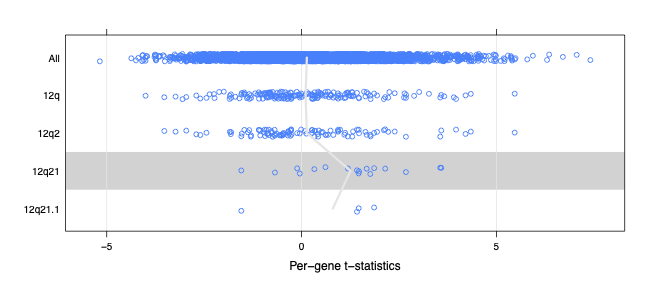
\includegraphics[width=.98\textwidth]{gseaStripplot}
\end{center}
\caption{ Per-gene $t$-statistics, as computed by \Rpackage{limma},
  for selected chromosome bands.  The points are jittered vertically
  to alleviate overlap.  A thick grey line joins the mean value within
  each group.  A GSEA test would compare the genes in 12q21 with those
  in 12q, or the entire gene universe, by fitting a linear model with
  per-gene $t$-statistics as the response, and a term indicating
  membership in 12q21 as the predictor.  If 12q21.1 is declared as
  significant, a conditional GSEA test would include an additional
  term for 12q21.1. }
\label{fig:gseaStripplot}
\end{figure}





We fit a factorial model to see whether the distribution of $y_i$ is
associated with category membership.  Specifically, for category $j$,
we fit the model
\begin{equation}
  \label{eq:lm1}
  y_i = \beta_0 + \beta_1 a_{ij} + \varepsilon_{i}
\end{equation}
where $a_{ij} = 1$ if gene $i$ belongs to category $j$, and $0$
otherwise.  The index $i$ may range over the full gene universe, or a
subset, depending on whether one wishes to perform global or local
tests.  The null hypothesis of no association is represented by $H_0:
\beta_1 = 0$.  The model nominally assumes that the $y_i$-s are
Normally distributed with equal variance, but in practice the results
are robust against mild deviations.  The presence of an intercept term
allows nonzero overall mean, which can be important in many
situations, especially for local tests.  We expect the test to be
fairly insensitive to distributional assumptions on the $y_i$-s.


We can fit (\ref{eq:lm1}) by least squares and test $H_0: \beta_1 = 0$
to obtain a marginal test for each category $j$; in this case, each
chromosome band.  The procedure also generalizes to incorporate the
nesting structure of chromosome bands.  Specifically, if band $j_2$
(e.g., 12q21.1) is nested within a coarser band $j_1$ (e.g., 12q21)
and the more granular band $j_2$ is significant, then the effect of
membership in $j_1$ over and above the effect attributable to
membership in $j_2$ can be tested by fitting the model
\begin{equation}
  \label{eq:lm2}
  y_i = \beta_0 + \beta_1 a_{ij_1} + \beta_2 a_{ij_2} + \varepsilon_{i}
\end{equation}
and testing the null hypothesis $H_0: \beta_1 = 0$.  Multiple
significant sub-bands and multiple levels of nesting can be
incorporated by including further terms in the model.  The complete
process can be summarized as follows: Start by marginally testing each
band which has no sub-bands.  For all other bands, first test all
sub-bands, then test the current band using a linear model that
includes a term for each \emph{significant} sub-band.

We apply this procedure to perform global tests using per-gene
$t$-statistics as a measure of differential expression in BCR/ABL
relative to NEG samples.  As with the Hypergeometric tests, we start
by creating objects of class \Rclass{ChrMapLinearMParams}.
%
\begin{Schunk}
\begin{Sinput}
> params <- new("ChrMapLinearMParams",
+               conditional = FALSE,
+               testDirection = "up",
+               universeGeneIds = entrezUniverse,
+               geneStats = tstats,
+               annotation = "hgu95av2",
+               pvalueCutoff = 0.01, 
+               minSize = 4L)
> params@graph <- makeChrBandGraph(params@annotation, params@universeGeneIds)
> params@gsc <- makeChrBandGSC(params@graph)
> paramsCond <- params
> paramsCond@conditional <- TRUE
\end{Sinput}
\end{Schunk}
The tests are performed, and the results summarized by
\begin{Schunk}
\begin{Sinput}
> lmans <- linearMTest(params)
> lmansCond <- linearMTest(paramsCond)
> chrSortOrder(summary(lmans))
\end{Sinput}
\begin{Soutput}
     ChrMapID       Pvalue    Effect Size Conditional TestDirection
53      12q21 1.226213e-03 1.1250647   17       FALSE            up
54    12q21.3 7.675013e-03 1.8539775    4       FALSE            up
76         14 6.053485e-03 0.3117778  157       FALSE            up
77        14q 6.053485e-03 0.3117778  157       FALSE            up
81       14q2 2.305207e-04 0.6152527   77       FALSE            up
83      14q22 1.153599e-04 1.2608760   20       FALSE            up
98      15q21 7.864796e-03 0.8721684   18       FALSE            up
133       18p 1.034270e-03 0.8925126   28       FALSE            up
134      18p1 1.034270e-03 0.8925126   28       FALSE            up
135     18p11 1.034270e-03 0.8925126   28       FALSE            up
137   18p11.3 5.687826e-03 1.0748058   13       FALSE            up
161       1p2 3.768696e-03 0.7247847   32       FALSE            up
162      1p21 8.355225e-04 1.5208019   10       FALSE            up
216         2 4.064842e-04 0.3060445  300       FALSE            up
227        2q 1.249084e-04 0.4364493  171       FALSE            up
228       2q1 9.527008e-03 0.5694083   40       FALSE            up
237       2q3 4.820761e-03 0.4063168   97       FALSE            up
240      2q33 7.529350e-03 0.9032265   17       FALSE            up
243         3 1.402517e-03 0.3008901  244       FALSE            up
256        3q 1.919247e-04 0.4981449  122       FALSE            up
263       3q2 2.371159e-03 0.4366903  100       FALSE            up
266      3q25 3.809785e-04 1.2148855   18       FALSE            up
271         4 9.538389e-04 0.3844196  158       FALSE            up
277        4q 4.601941e-03 0.3844843  110       FALSE            up
279      4q13 6.143774e-03 0.9302421   17       FALSE            up
291         5 1.089529e-03 0.3350615  205       FALSE            up
297        5q 5.954123e-03 0.2982655  173       FALSE            up
303       5q2 5.551978e-03 0.8926298   19       FALSE            up
306      5q23 3.555656e-03 1.6809836    6       FALSE            up
311         6 1.584787e-04 0.3432447  274       FALSE            up
322        6q 6.962197e-06 0.6880899   95       FALSE            up
326       6q2 5.900992e-06 0.8116250   69       FALSE            up
330      6q24 3.202752e-03 1.5764875    7       FALSE            up
348    7q21.1 9.147762e-03 1.1422131   10       FALSE            up
385        9q 6.018718e-03 0.3690938  111       FALSE            up
387      9q21 2.799870e-04 1.2451339   18       FALSE            up
388    9q21.1 4.282873e-06 2.1509042   10       FALSE            up
1042 10p11.22 8.053864e-03 1.8405737    4       FALSE            up
1174  14q22.2 9.092615e-06 2.6734149    6       FALSE            up
1205  15q24.3 8.504394e-03 1.6328169    5       FALSE            up
1220  16q12.1 7.610085e-03 1.4037361    7       FALSE            up
1254 18p11.22 1.003528e-03 1.6707653    8       FALSE            up
1293   1p21.3 2.500404e-03 1.7529252    6       FALSE            up
1503   4q13.3 8.388741e-03 1.0570420   12       FALSE            up
1577   6p22.3 2.989781e-03 1.1672122   13       FALSE            up
1594     6q21 1.292155e-03 1.1191866   17       FALSE            up
1598   6q23.3 3.192526e-03 1.5770967    7       FALSE            up
1600   6q24.2 7.434128e-03 1.8628060    4       FALSE            up
1631   7q31.2 4.049223e-05 2.6936729    5       FALSE            up
1686  9q21.13 7.571655e-04 1.9803350    6       FALSE            up
1700   9q33.2 3.825568e-04 2.1006502    6       FALSE            up
\end{Soutput}
\begin{Sinput}
> chrSortOrder(summary(lmansCond))
\end{Sinput}
\begin{Soutput}
     ChrMapID       Pvalue    Effect Size Conditional TestDirection
54    12q21.3 7.675013e-03 1.8539775    4        TRUE            up
81       14q2 7.893819e-03 0.4407200   77        TRUE            up
98      15q21 7.864796e-03 0.8721684   18        TRUE            up
137   18p11.3 5.687826e-03 1.0748058   13        TRUE            up
228       2q1 9.527008e-03 0.5694083   40        TRUE            up
240      2q33 7.529350e-03 0.9032265   17        TRUE            up
256        3q 6.983745e-03 0.3725591  122        TRUE            up
266      3q25 3.809785e-04 1.2148855   18        TRUE            up
271         4 5.357453e-03 0.3282355  158        TRUE            up
291         5 3.987179e-03 0.2940783  205        TRUE            up
306      5q23 3.555656e-03 1.6809836    6        TRUE            up
348    7q21.1 9.147762e-03 1.1422131   10        TRUE            up
388    9q21.1 8.243858e-04 2.4034672   10        TRUE            up
1042 10p11.22 8.053864e-03 1.8405737    4        TRUE            up
1174  14q22.2 9.092615e-06 2.6734149    6        TRUE            up
1205  15q24.3 8.504394e-03 1.6328169    5        TRUE            up
1220  16q12.1 7.610085e-03 1.4037361    7        TRUE            up
1254 18p11.22 1.003528e-03 1.6707653    8        TRUE            up
1293   1p21.3 2.500404e-03 1.7529252    6        TRUE            up
1503   4q13.3 8.388741e-03 1.0570420   12        TRUE            up
1577   6p22.3 2.989781e-03 1.1672122   13        TRUE            up
1594     6q21 1.292155e-03 1.1191866   17        TRUE            up
1598   6q23.3 3.192526e-03 1.5770967    7        TRUE            up
1600   6q24.2 7.434128e-03 1.8628060    4        TRUE            up
1631   7q31.2 4.049223e-05 2.6936729    5        TRUE            up
1686  9q21.13 7.571655e-04 1.9803350    6        TRUE            up
1700   9q33.2 3.825568e-04 2.1006502    6        TRUE            up
\end{Soutput}
\begin{Sinput}
> 
> ##
\end{Sinput}
\end{Schunk}
%%
These examples only test for consistently upregulated categories;
similar calls with \texttt{testDirection = "down"} can be used to test
for downregulation.  As we see, the GSEA approach picks out many more
bands as significant, but there is some concordance with the
Hypergeometric approach.  For example, 7q31, 8p22, and 14q22.2 come up
in both analyses.  Figure~\ref{fig:dotplot1p362} shows box-and-whisker
plots of genes in one category (1p36.2) that is declared as
significant by the Hypergeometric test, but not by GSEA.  It is
produced by
\begin{Schunk}
\begin{Sinput}
> tmpSet <- subsetByBand(nsFiltered, ct, "1p36.2")
> esetBWPlot(tmpSet, ylab="1p36.2", layout = c(2, 8),
+            par.strip.text = list(cex = 0.8))
\end{Sinput}
\end{Schunk}
%
\begin{figure}[tb]
\begin{center}
  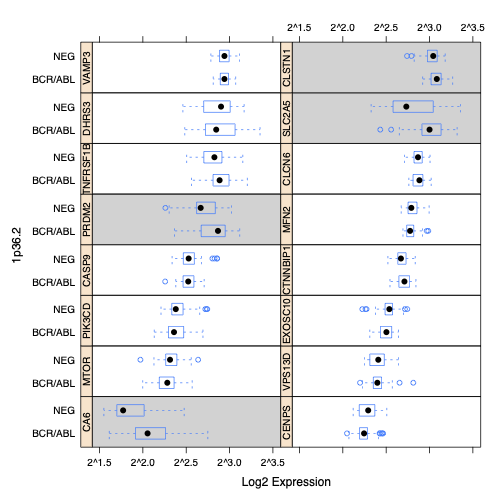
\includegraphics[width=.98\textwidth]{dotplot1p362}
\end{center}
\caption{Expression values for the BCR/ABL and NEG samples for the
  genes located within 1p36.2, which is declared as significant by the
  Hypergeometric test, but not by GSEA.  Genes in the selected list
  are highlighted with a shaded background.  For these genes, The NEG
  samples, those with no known cytogenetic abnormalities, have
  significantly lower expression than the BCR/ABL samples.  However,
  the direction is reversed (albeit mildly) for many of the other
  genes.  }

\label{fig:dotplot1p362}
\end{figure}


\bibliography{cat}


\end{document}

